\documentclass{article}
\usepackage[margin=2cm]{geometry}
\usepackage{amsmath, amsfonts, amsthm}
\usepackage{xcolor}
\usepackage{enumerate}
\usepackage{graphicx}

\theoremstyle{definition}
\newtheorem*{definition}{Definition}
\newtheorem{theorem}{Theorem}
\newtheorem{corollary}{Corollary}
\newtheorem{assumption}{Assumption}

\newcommand{\ah}[1]{\textcolor{blue}{AH: \textit{#1}}}
\newcommand{\fb}[1]{\textcolor{red}{FB: \textit{#1}}}

\newcommand{\agentset}{\mathcal{N}}
\newcommand{\edgeset}{\mathcal{E}}
\newcommand{\weightset}{W}

\newcommand{\actionset}[1]{S^{#1}}
\newcommand{\utility}[1]{u^{#1}}

\newcommand{\wmunu}{w^{\mu \nu}}
\newcommand{\xmu}{x^{\mu}}
\newcommand{\xnu}{x^{\nu}}
\newcommand{\refmu}{\sigma^{\mu}}
\newcommand{\avgref}[1]{\alpha_\sigma^{#1}}
\newcommand{\NE}[1]{\bar{x}^{#1}}
\newcommand{\weightedsum}{ \sum_{\nu \in N^\mu} \wmunu \xnu}
\newcommand{\xnotmu}{x^{-\mu}}
\newcommand{\xmuaction}[1]{x^{\mu}_{#1}}


\title{Fictitious Play in Network Aggregative Games}
\author{AH, FB}

\begin{document}
	
	\maketitle

	\section{Paper Structure}

	\begin{enumerate}
		\item Introduction: Explain the notion of a Network Aggregative Game, and Fictitious Play
		with literature on the state of the art. Assumptions made as well as summary of results
		\item Maybe? Relation with the model of Grammatico
		\item Preliminaries \begin{itemize}
			\item The Network Aggregative Game model
			\item Fictitious Play, as well as the CTFP property
		\end{itemize}
		\item Convergence of Fictitious Play \begin{itemize}
			\item Existence of the Nash Equilibrium
			\item Existence of a CTFP
			\item Convergence of CTFP to a fixed point
			\item Corrolary: when $w_{ii} = 0$ (i.e. the interaction graph is simple) CTFP converges
			to a NE
			\item Convergence of CTFP to the NA-CCE set
		\end{itemize}
		\item Numerical Experiments \begin{itemize}
			\item Non-convergent examples
			\item Fictitious Play with Noise
		\end{itemize}
		\item Discussion of Experiments
		\item Concluding Remarks
	\end{enumerate}
	
	\newpage
	\section{Introduction}
<<<<<<< HEAD


=======
		

>>>>>>> 419ff6d149a62469e9028a7c9ecc84a8ae5d8a22
		\subsection{Contributions}

		The main contribution of this work is to study the
                behaviour of the Fictitious Play Learning Algorithm,
                in continuous time, when applied on a Network
                Aggregative Matrix Game.
\fb{why FP and NAG are important?}


                We first show that a Nash
                Equilibrium exists and that Fictitious Play admits
                solutions in this setting. In particular, we study
                zero-sum games and show that Fictitious Play converges
                to a fixed point, which for a network without any self-loops
                corresponds to a Nash Equilibrium. In addition, we
                find that, for games which are not zero-sum, agents
                following Continuous Time Fictitious Play are able to
                achieve no regret.

		Finally, we explore the Fictitious Play algorithm
                through numerical simulations to understand how
                convergence rates depend on the network size and
                connectivity. We also show that it does not
                necessarily converge for more complex games and can,
                in fact, lead to more complex dynamics. In addition,
                we experiment the Fictitious Play algorithm on an
                agent based model for \ah{resource allocation? 
                voting?}. Finally, our experiments document how noise
                affects the convergence of fictitious play, whose
                theoretical analysis we point out as an interesting
                direction for future work.

		\ah{Possible additions: 1) Show that the flow is
                  unique almost everywhere in CTFP. 2) Show the same
                  results (i.e. existence and convergence) for
                  Discrete Time Fictitious Play.}


<<<<<<< HEAD
	\subsection{Related Work}
		Main articles: 
		\begin{enumerate}
			\item Ewerhart (FP in Networks). Main difference is in the model we consider - i.e. agents only track the aggregate strategy rather than strategies of all neighbours. Further, our analysis shows that in non-simple networks, FP still converges to a fixed point, although not an NE.
			\item Grammatico (NE seeking in NA games). Main difference is that we look at the case where the payoffs are bilinear (since in matrix form), so that we need to consider best response correspondences rather than assuming a unique minimiser.
			\item Perrin (FP in Mean Field Games). Main difference is that we assume an underlying communication network rather than assuming that the players play against the entire population (which is a special case of our analysis, in which you assume that all players are connected to each other).
			\item Sela (FP in one-against-all networks) Similarly, this paper doesn't assume an underlying communication network or any form of weighted communication between the agents.
		\end{enumerate}
=======
		\subsection{Related Work}
					Main articles: 
					\begin{enumerate}
						\item Ewerhart (FP in Networks). Main difference is in the model we consider - i.e. agents only track the aggregate strategy rather than strategies of all neighbours. Further, our analysis shows that in non-simple networks, FP still converges to a fixed point, although not an NE.
						\item Grammatico (NE seeking in NA games). Main difference is that we look at the case where the payoffs are bilinear (since in matrix form), so that we need to consider best response correspondences rather than assuming a unique minimiser.
						\item Perrin (FP in Mean Field Games). Main difference is that we assume an underlying communication network rather than assuming that the players play against the entire population (which is a special case of our analysis, in which you assume that all players are connected to each other).
						\item Sela (FP in one-against-all networks) Similarly, this paper doesn't assume an underlying communication network or any form of weighted communication between the agents.
					\end{enumerate}
>>>>>>> 419ff6d149a62469e9028a7c9ecc84a8ae5d8a22
                
		\section{Preliminaries}
	\subsection{Network Aggregative Games}
	\label{sec::NAG}

	The model we consider is that there is a set $\agentset = {1,
         \ldots , N}$ of agents who are connected through an underlying
        interaction graph. This graph is given by the tuple
        $(\agentset, (\edgeset, \weightset))$ in which $\edgeset$ is
        the set of all pairs $(\mu, \nu) \in \agentset \times
        \agentset$ such that agent $\mu$ and agent $\nu$ are
        connected. Formally,
        
          \begin{definition}[Interaction Graph]
  Given a set $\agentset$ of agents, an {\em interaction graph} $I = (\agentset, (\edgeset, \weightset))$ such that
  \begin{itemize}
  \item $\edgeset \subseteq \agentset \times \agentset$.        Then, the set of neighbours of agent $\mu$ is
        denoted as $N^\mu = \{\nu \in \agentset \, : \, (\mu, \nu) \in
        \edgeset\}$.
    \item $\weightset \in M_N(\mathbb{R})$ is the weighted
        adjacency matrix whose elements $w^{\mu \nu}$ expresses the
        importance that agent $\mu$ places on agent $\nu$. If $(\mu, \nu) \not \in \edgeset$ then $w^{\mu \nu} = 0$;        $\wmunu \in (0, 1]$ otherwise.
  \end{itemize}
\end{definition}


	As a network game, each agent $\mu$ has an associated set of
        actions $\actionset{\mu}$ which has cardinality
        $|\actionset{\mu}| = n$. \fb{what is a strategy then? how can
          we define them if we didn't introduce actions?}


        We can construct the \fb{unit-simplex ?} on the action
        set as $\Delta_\mu := \{x \in \mathbb{R}^n \, : \, \sum_i
        \xmuaction{i} = 1\}$ where $\xmuaction{i}$ is the probability
        with which agent $\mu$ plays the action $i$. As such we
        refer to $\xmu$ as the \emph{state} of agent $\mu$ (this is
        often referred to as $\mu$'s mixed strategy). Also associated
        with each agent is a utility function $u^\mu(\xmu, \xnotmu)$
        in which we use the standard notation $-\mu$ to refer to all
        agents other than $\mu$. Notice that this requires that each
        agent plays the same strategy against all of their neighbours.

	With all of the above definitions, we can formalise the
        network aggregative (NA) game:
	
	\begin{definition}[Network Aggregative Game]
		A Network Aggregative game is defined as the tuple $\Gamma =
        (\agentset, (\edgeset, \weightset), (\actionset{\mu},
        \utility{\mu})_{\mu \in \mathcal{N}})$, where $\agentset$, $\edgeset$, $\weightset$ are as
        defined in the Interaction graph. $\actionset{\mu}$ and $\utility{\mu}$ refer to the set of
        actions and the utility function of agent $\mu$ respectively..
	\end{definition}


	What is unique about the NA game is the structure of the
        payoffs themselves. In this format, each agent is receives a
        reference $\sigma$ which is a weighted sum of each of their
        neighbours state. Formally
%
	\begin{equation}
		\sigma^\mu = \sum_{\nu \in N^\mu} \wmunu \xnu.
	\end{equation}

	Then, the agent's must optimise their payoff with respect to
        this reference vector. Thus, instead of having to consider the
        actions of the entire population, or play individual games
        against each of their neighbours, the agent only has to
        consider $\sigma^\mu$ as a `measurement' of the local
        aggregate state and optimise with respect to this
        measurement. This allows us to make the reduction $u^\mu(\xmu,
        \xnotmu) = u^\mu(\xmu, \refmu)$. In particular, we consider
        that the agent is engaged in a matrix game against the
        reference vector so that
%
	\begin{equation}
		u^\mu(\xmu, \refmu) = \xmu \cdot A^\mu \refmu = \xmu
                \cdot A^\mu \weightedsum.
	\end{equation}
	where $A^\mu$ is the payoff matrix associated to agent
        $\mu$. Note that this means we can write the game
        $\Gamma$ with the payoff matrices $A^mu$ in place of the
        utility functions $\utility{\mu}$. The NA game allows for the
        reduction of a multiplayer game into a series of two-player
        games. The agent's goal is to maximise their payoff with
        respect to the reference vector. As such, we define the best
        response correspondence $BR^\mu$ which maps any $\refmu$ the
        set $\arg \max_{y \in \Delta_\mu} {u^\mu(y, \refmu)}$. This
        leads naturally to the definition of a Nash Equilibrium in an
        NA Game as

	\begin{definition}(NE)
		The set of vectors $\{ \NE{\mu}\}_{\mu \in \agentset}$ is an NE if, for all $\mu$,	
		\begin{equation*}
		\NE{\mu} \in \arg \max_{x \in \Delta_\mu} u^\mu(x, w^{\mu \mu} x + \sum_{\nu \in N^\mu \backslash \{\bar{\mu}\}} \wmunu \NE{\nu}).
		\end{equation*}	
	\end{definition}
        \fb{It this a definition or rather a lemma?}

	We will show that such an equilibrium exists in .... Finally we note that an NA game is \emph{zero-sum} if the utilities of each agent sum to zero for any strategy set $\{ \xmu \}_{\mu \in \agentset}$. Formally

	\begin{equation}
		\sum_\mu u^\mu(\xmu, \weightedsum) = 0.
	\end{equation}

	\subsection{Continuous Time Fictitious Play}
	\label{sec::CTFP}

	\ah{For Francesco: is it worth giving a quick introduction to Fictitious Play by talking about two player games?}
\fb{I'd rather give the definition first and then the example.}
        

	Fictitious Play requires that, at the current time, each agent
        considers the average behaviour of their opponent in the past
        and play a best response to that strategy. This is best
        illustrated in the two-player setting. Consider the two player
        normal form game $\Gamma_2 = (\{ 1, 2\}, ((S^1, A), (S^2,
        B)))$ so that $A$ and $B$ are the payoff matrices of agent $1$
        and $2$ respectively. As a remark, note that we can write the
        two player normal form game as an NA game simply by requiring
        that $\edgeset = \{(1, 2), (2, 1)\}$ and $\weightset$ is a 2x2
        matrix with zeros on its leading diagonal and ones on the off
        diagonal. We write the time-average of both agents' strategies
        as
%
	\begin{align}
		\alpha^i = \frac{1}{t} \int_0^T x^i(t) \, dt & \text{ for $i \in \{1, 2\}$}
%		\alpha^2 = \frac{1}{t} \int_0^T x^2(t) \, dt \\
	\end{align}
        \fb{why using an integral rather than a simple summation?}

        \fb{decide whether you start enumerations from 1 or 0.}


	In this manner, the $\alpha^\mu(t)$ denotes the time average of the strategies played by agent
	$\mu$ up to time $t$. Then, fictitious play requires that the agents update their strategy as
	$x^1(t) \in BR^1(\alpha^2(t))$ and $x^2(t) \in
	BR^2(\alpha^1(t))$. 

	We extend this naturally to the NA game $\Gamma$ by requiring that each agent update their
	strategy according to the time average of their reference vector $\refmu$. To formalise this, we
	write
	\begin{equation}
		\avgref{\mu} = \frac{1}{t} \int_0^t \refmu(s) \; ds.
	\end{equation}

	Using this, we follow in the footsteps of Ewerhart \cite{} and Harris \cite{} to define
	Fictitious Play in continuous time.
%
	\begin{definition}[Continuous Time Fictitious Play (CTFP)]
		A CTFP is defined as a measurable map $m$ with components $m_i$ such that for all $i$ and
		all $t \geq 1$, $m_i: [0, \infty) \rightarrow \Delta_i$ satisfies $m_i(t) \in
		BR_i(\alpha_{\sigma_i})$ for almost all $t \geq 1$.
	\end{definition}

		We can think of this definition as saying that the player plays some arbitrary strategy before $t = 1$, but beyond this it must play a best response to the time average of its reference signal.

	\subsection{Assumption}

	With the above preliminaries in place, we can state the assumptions that we make in this study.

	\begin{assumption}
		The weighted adjacency matrix $\weightset$ is constant and \emph{row stochastic} meaning
		that the sum elements in each row of $\weightset$ is equal to one.
	\end{assumption}

	\begin{assumption}
		The payoffs are given through matrix games and, therefore, are bilinear.
	\end{assumption}

	\begin{assumption}
		The cardinality of each action set $|\actionset{\mu}|$ is equal for all agents.
	\end{assumption}

	\begin{assumption}
		The NA game is zero-sum in the sense that $\sum_{\mu} u^\mu(\xmu, \weightedsum)$ for any set
		of states $(x^\mu)_{\mu \in N^\mu}$
	\end{assumption}

\fb{discuss how restrictive each of these assumptions is.}
        

	\section{Convergence of Fictitious Play}

	\subsection{Existence of the Nash Equilibrium}
	
	Note that the NE Condition requires

	\begin{align}
		\NE{\mu} &\in \arg\max_{x \in \Delta_\mu} u^\mu(x, w^{\mu \mu}x + \sum_{\nu \in N^\mu} w^{\mu \nu} \NE{\nu}) \nonumber \\
		& =: \arg\max_{x \in \Delta_i} \bar{u}^\mu(x, \sum_{\nu \in N^\mu} w^{\mu \nu} \NE{\nu})
	\end{align}

	where we can find $\bar{u}_i$ through the following argument
	
	\begin{align}
		u^\mu(x, w^{\mu \mu} x + \sum_{\nu \in N^\nu} w_{\mu \nu} \NE{\nu}) & = x \cdot A^\mu (w^{\mu \mu} x + \sum_{\nu \in N^\mu} w_{\mu \nu} \NE{\nu}) \\
		 & = x \cdot (w^{\mu \mu} A^\mu)  x + \sum_{\nu \in N^\mu} u^{\mu \nu}(x, \NE{\nu}) \\
		 & =: \bar{u}^\mu(x, \sum_{\nu \in N^\mu} w^{\mu \nu} \NE{\nu}), \nonumber
	\end{align}
	
	where $u^{\mu \nu}(\xmu, x^\nu) = \xmu \cdot A^\mu x^\nu$. Note that, in order to get this
	formulation, we had to use the assumption of payoffs being bilinear so that we could separate
	out the term in the weighted sum involving $x$ from $\bar{x}^\nu$. 
	
	To show existence of an NE we will need the following definition and theorem.

	\begin{definition}[Upper Semi-Continuous]
		A compact-valued correspondence $\Phi: A \rightarrow B$ is \emph{upper semi-continuous} at a point $a$ if $g(a)$ is non-empty and if, for every sequence $a_n \rightarrow a$ and every sequence $(b_n)$ such that $b_n \in g(a_n)$ for all $n$, there exists a convergent subsequence of $(b_n)$ whose limit point $b$ is in $g(a)$.  
	\end{definition}

	\begin{theorem}[Kakutani]
		Let $K \subset \mathbb{R}^n$ be compact and convex and $\Phi: K \rightarrow K$ be closed or upper semi-continuous, with nonempty, convex and compact values. Then $\Phi$ has a fixed point.
	\end{theorem}

	Note that, when acting on a simplex, the function $\Phi: \Delta \rightarrow \textbf{P}(\Delta)$, where $\textbf{P}(\Delta)$ denotes the nonempty, closed and convex subsets of $\Delta$ only has to satisfy the upper-semi continuity condition to admit a fixed point.

	\begin{theorem}[Existence of NE]
		Under the assumption (II), namely that the payoff function achieves a bilinear property, a
		Nash Equilibrium $\{\bar{x}^\mu\}_{\mu \in \agentset}$ exists.
	\end{theorem}

	\begin{proof}
		We begin by rewriting the NE condition by concatenating the set of NE vectors into one long colunn vector. This gives

		\begin{equation}
			\begin{bmatrix}
				\bar{x}^1 \\ . \\ . \\ . \\ \bar{x}^N
			\end{bmatrix} \in
			\begin{bmatrix}
			\arg\max_{y \in \Delta_1} \bar{u}^1(y, \sum_{\nu \in N^1} w^{1 \nu} \bar{x}^\nu) \\ . \\ . \\ . \\ \arg\max_{y \in \Delta_N} \bar{u}^1(y, \sum_{\nu \in N^N} w^{N \nu} \bar{x}^\nu)
			\end{bmatrix}	.
		\end{equation}

		We can rewrite the weighted summation for $\mu$ as

		\begin{equation}
			\sum_{\nu \in N^\mu} w^{\mu \nu} \bar{x}^\nu = (w_{-\mu}^T \otimes I_n) \begin{bmatrix}
				\bar{x}^1 \\ . \\ . \\ . \\ \bar{x}^N
			\end{bmatrix},
		\end{equation}
	
		in which $w_{-\mu}$ is a column vector containing $w^{\mu \nu}$ in the $\nu$'th element for all $j \in N^\mu$ and 0 everywhere else (including in the $\mu$'th slot), $I_n$ is the $n \times n$ identity matrix and $\otimes$ is the kronecker product. For example, the form for agent 1, in the case of 2-action game is given by

		\begin{equation}
			(w_{-1}^T \otimes I_2) = [0, w_{12}, w_{13}, ..., w_{1n}] \otimes I_2 = 
			\begin{bmatrix}
				0 & 0 & w_{12} & 0 & ... & w_{1n} & 0 \\
				0 & 0 & 0 & w_{12} & ... & 0 & w_{1n} \\
			\end{bmatrix}
		\end{equation}
		
		Returning to the $N$-player NA game our condition becomes
		\begin{equation}
			\begin{bmatrix}
				\NE{1} \\ . \\ . \\ . \\ \bar{N}
			\end{bmatrix} \in
			\begin{bmatrix}
				\arg\max_{y \in \Delta_1} \bar{u}^1(y, (w_{-1}^T \otimes I_n) \begin{bmatrix}
					\NE{1} \\ . \\ . \\ . \\ \NE{N}
				\end{bmatrix}) \\ . \\ . \\ . \\ \arg\max_{y \in \Delta_N} \bar{u}_N(y, (w_{-N}^T \otimes I_n) \begin{bmatrix}
				\NE{1} \\ . \\ . \\ . \\ \NE{N}
			\end{bmatrix}))
			\end{bmatrix}	.
		\end{equation}

		This means that we achieve a Nash Equilibrium iff $(\NE{\mu})_{\mu \in \agentset}$ is a fixed point of the map
	
	
		\begin{equation}
			\begin{bmatrix}
				\arg\max_{y \in \Delta_1} \bar{u}^1(y, (w_{-1}^T \otimes I_n) ( \cdot )) \\ . \\ . \\ . \\ \arg\max_{y \in \Delta_N} \bar{u}^N(y, (w_{-N}^T \otimes I_n)( \cdot ))
			\end{bmatrix}	.
		\end{equation}


		Now, since the modified payoff $\bar{u}^\mu$ shares the same bilinear property as $u^\mu$, we can assert that it is continuous is its second argument. Therefore, the above vector valued map can be asserted to be continuous and so is upper semi-continuous. As such, we can apply Kakutani's Fixed Point Theorem to assert that the above map admits a fixed point.

	\end{proof}

	\subsection{Existence of CTFP}

	\begin{theorem}
		There exists a path $m$ which satisfies the property that, for all $\mu$, $m^\mu \in
		BR^\mu(\alpha_\sigma^\mu)$ for almost aall $t \geq 1$.
	\end{theorem}

	\begin{proof}
		Recall the definition of $\alpha^\mu(t)$

		\begin{equation*}
		\alpha^\mu(t) = \frac{1}{t} \int_{0}^{t} m^\mu(s) \, ds
		\end{equation*}

		Then 

		\begin{align}
		\frac{d}{dt} \alpha^\mu(t) & = \frac{d}{dt} \frac{1}{t} \int_{0}^t m^\mu(s) ds \nonumber \\
		& = \frac{1}{t} m^\mu(t) - \frac{1}{t} \alpha^\mu(t)
		\end{align}

		Now we assert that $m^\mu(t) \in BR^\mu(\alpha_{\sigma}^\mu) = \arg\max_{y \in \Delta_\mu} u^\mu(y,
		w^{\mu \mu} \alpha^\mu(t) + \sum_{\nu \in N^\mu} w_{ij} \alpha^\nu(t))$. 

		Let us then define $\alpha(t)$ as the concatenation of all $\alpha_i(t)$

		\begin{equation}
			\alpha(t) = \begin{bmatrix}
				\alpha^1(t)^T, \ldots, \alpha^N(t)^T
			\end{bmatrix}^T \subset \mathbb{R}^{Nn}
		\end{equation}


		We can, therefore, write the aggregation as

		\begin{equation}
			(W \otimes I_n) \alpha(t) = \begin{bmatrix}
				\sum_{\nu \in N^1} w^{1 \nu} \alpha^\nu(t) \\
				.\\
				.\\
				.\\
				\sum_{\nu \in N^N} w^{N \nu} \alpha^\nu(t)
			\end{bmatrix} \subset \mathbb{R}^{Nn}
		\end{equation}

		I will write $(W \otimes I_n) \alpha(t)$ as $\alpha_W$ for convenience. Furthermore, using
		the bilinear property of the game, we can say that

		\begin{equation}
			\begin{bmatrix}
				\arg\max_{y_1 \in \Delta_1} y \cdot A^1 ( \alpha_W(t))_1 \\
				.\\
				.\\
				.\\
				\arg \max_{y_N \in \Delta_N} y \cdot A^N (\alpha_W(t))_N 
			\end{bmatrix} = 
			\arg \max_{y \in \Delta} y \cdot \begin{bmatrix}
				A^1 & 0 & . & . & . & 0 \\
				0 & A^2 & . & . & . & 0 \\
				& & . & & & \\
				& & & . & & \\
				& & & & . & \\
				0 & 0 & . & . & . & A^N \\
			\end{bmatrix} \alpha_W(t) = \arg\max_{y \in \Delta} y \cdot \Lambda (W \otimes I_n)
			\alpha(t)
		\end{equation}

		in which $\Delta = \times_i \Delta_i$ and $\Lambda$ is the block diagonal matrix containing
		each $A^i$. 

		We can now write the differential inclusion as

		\begin{equation}
			\dot{\alpha}(t) \in \frac{1}{t} (\arg \max_{y \in \Delta}  \{y \cdot \Lambda (W \otimes
			I_n)
			\alpha(t) \}- \alpha(t))
		\end{equation}

		with the initial condition $\alpha(1) = x_0$. Then, the path $m$ is a CTFP if its
		corresponding $\alpha(t; m)$ is a solution to the above differential inclusion. Following
		the definition of (Harris 1998), a solution $\alpha(t)$ must satisfy

		\begin{enumerate}
			\item $\alpha(t)$ is locally Lipschitz
			\item $\alpha(1) = x_0$
			\item $\dot{\alpha}(t) \in \frac{1}{t} (\arg \max_{y \in \Delta}  \{y \cdot \Lambda (W \otimes
			I_n)
			\alpha(t) \}- \alpha(t))$ for almost all $t \in [1, \infty)$ 
		\end{enumerate}

		The question then remains, does the differential inclusion admit a solution? Using the
		results of Aubin and Cellina (see Harris 1998, paragraph below Prop. 6), can use the fact
		that the $\arg \max$ function is non-empty, compact and convex valued, bounded (all of
		these follow since the function acts from $\Delta$ to $\Delta$) and upper semi-continuous. 
		With these facts in place, we can say that there is a CTFP $m$ for any initial value $x_0$. Further, the solution $m(t)$ is Lipschitz for almost all $t \geq 0$.

	\end{proof}

	With the existence of the CTFP in place, we can show that it converges to a fixed point. In particular, let $\Omega(\alpha)$ be the set of all limit points for $\alpha(t)$. Then, a CTFP path is said to have converged if $\Omega(\alpha)$ is contained within the set of Nash Equilibria of the game. If this is for any such CTFP path, then the game is said to have the \emph{CTFP property}. We adapt the techniques of (Ewerhart 2020) to prove that zero-sum NA games have the CTFP property. \ah{I also want to attempt this with the techniques of Harris (which is quite similar) to see if it yields any new results}.

	\begin{theorem}
		Any zero-sum NA game has the property that, for any CTFP path $m$, the corresponding $\alpha(t; m)$ converges to a set of fixed points.
	\end{theorem}


	\begin{proof}

		\begin{equation}
			m^\mu(t) \in BR^\mu \left( \frac{1}{t} \int_{0}^{t} \sigma^\mu(s) ds \right).
		\end{equation}
		
		By the definition of Continuous Time Fictitious Play (CTFP) given by Ewerhart, we require that $m: [0, \infty) \rightarrow \times_\mu \Delta_\mu$ is a measurable mapping such that, for each $\mu$, $m^\mu(t) \in BR^\mu \left( \frac{1}{t} \int_{0}^{t} \sigma^\mu(t') dt' \right)$. Now notice,
		
		\begin{equation*}
			m^\mu(t) \in BR^\mu \left( \frac{1}{t} \int_{0}^{t} \sigma^\mu(t') dt' \right) \iff  \in x^\mu\in BR^\mu \left( \frac{1}{t} \int_{0}^{t} [w^{\mu \mu} m^\mu(s) + \sum_{\nu \in N^\mu} w^{\mu \nu} m^\nu(s)] \, ds \right)
		\end{equation*}
		
		Let us assume that $u^\mu$ takes the form $x \cdot A^\mu \sigma^\mu$ where $A^\mu$ is the payoff matrix associated with agent $\mu$. Then,
		
		\begin{align}
			& m^\mu \in \arg\max_{x \in \Delta^\mu} u^\mu(x,\frac{1}{t} \int_{0}^{t} [w^{\mu \mu} m^\mu(t') + \sum_{\nu \in N^\mu} w^{\mu \nu} m^\nu(s)] \, ds) \nonumber \\
			\iff & m^\mu \in \arg\max_{x \in \Delta_\mu} x \cdot A^\mu \left(\frac{1}{t} \int_{0}^{t} [w^{\mu \mu} m^\mu(t') + \sum_{\nu \in N^\mu} w^{\mu \nu} m^\nu(s)] \, ds \right) \nonumber \\
			\iff & m^\mu \in \arg \max_{x \in \Delta_\mu} x \cdot (w^{\mu \mu} A^\mu) \left( \frac{1}{t} \int_{0}^{t} m^\mu(s) ds\right) + \sum_{\nu \in N^\mu} x \cdot (\wmunu A^\nu) \left( \frac{1}{t} \int_{0}^{t} m^\nu(s) ds \right) \nonumber \\
			\iff & m^\mu \in \arg \max_{x \in \Delta_i} x \cdot A^{\mu \mu} \alpha^\mu(t; m) + \sum_{\nu \in N^\mu} x \cdot A^{\mu \nu} \alpha^\nu(t; m).
		\end{align}
		
		where each $A^{\mu \nu} = \wmunu A^\mu$ and $\alpha^\mu(t; m) =\frac{1}{t} \int_{0}^{t} m^\mu(s) ds$ as defined by Ewerhart. We can, therefore, think of the NA game as a network game in which each agent plays the same strategy against each of its neighbours, itself included. As such, any $m$ which satisfies the CTFP property for the equivalent network game also satisfies the CTFP requirement for the network aggregative game. 
		
		Continuing with this approach, let us look at the case where $\sum_\mu A^\mu = \textbf{0}_{n\times n}$ (i.e. a zero sum game). This means that $\sum_i u_i = 0$. Let $\xmu_\infty = \lim_{t \rightarrow \infty} \alpha^\mu(t; m)$. More specifically, $\xmu_\infty$ belongs to the set of accumulation points of $\alpha^\mu(\cdot; m)$ (which is set valued since the $BR^\mu$ map is set valued). To say that the game has `converged' we require that every $\xmu_\infty = (x^1_\infty, ... x^N_\infty)$ is an NE. \ah{I'll follow through the proof of Ewerhart for the sake of completeness: }
		
		Let us take the Lyapunov function
		
		\begin{equation}
			L(x) = \sum_\mu \max_{y \in \Delta_\mu} \{u^\mu(y, w^{\mu \mu} \xmu + \sum_{\nu \in N^\mu} \wmunu \xnu) - u^\mu(\xmu, w^{\mu \mu} \xmu + \sum_{\nu \in N^\mu} \wmunu \xnu) \}
		\end{equation}
		
		Using the same transformation as before:
		
		\begin{align}
			 u^mu(y, w^{\mu \mu} \xmu + \sum_{\nu \in N^\mu} w_{\mu \nu} \xnu) & =  y \cdot A^\mu (w^{\mu \mu} \xmu + \sum_{\nu \in N^\mu} \wmunu \xnu) \nonumber \\
			 & =  y \cdot (w^{\mu \mu} A^\mu) \xmu + \sum_{\nu \in N^\mu} y \cdot (\wmunu A^\mu) \xnu \nonumber \\
			  & =  \sum_{\nu \in N^\mu \cup \{\mu\}} y \cdot A^{\mu \nu} \xnu \nonumber 
		\end{align}
		
		Then,
		
		\begin{align}
		L(x) &= \sum_\mu \max_{y \in \Delta_\mu}\sum_{\nu \in N^\mu \cup \{\mu\}} y \cdot A^{\mu \nu} \xnu  - u^mu(\xmu, w^{\mu \mu} \xmu + \sum_{\nu \in N^\mu} w^{\mu \nu} \xnu) \} \nonumber \\
		&= \sum_\mu \max_{y \in \Delta_\mu} \{\sum_{\nu \in N^\mu \cup \{\mu\}} y \cdot A^{\mu \nu} \xnu  \} - \sum_\mu  u^\mu(\xmu, w^{\mu \mu} \xmu + \sum_{\nu \in N^\mu} w^{\mu \nu} \xnu) \nonumber \\
		&= \sum_\mu \max_{y \in \Delta_\mu} \{\sum_{\nu \in N^\mu \cup \{\mu\}} y \cdot A^{\mu \nu} \xnu  \} \nonumber 
		\end{align}
		
		where the last equality holds because $\sum_\mu u^\mu = 0$. Now, in parallel with (Ewerhart 2020) we recall that we defined $m^\mu(t)$ as the best response to $\alpha(t)$. As such,

		\begin{align}
			L(\alpha(t)) & = \sum_\mu \sum_{\nu \in N^\mu \cup \{\mu\}} m^\mu(t) \cdot A^{\mu \nu} \alpha^\nu(t) \\
			t L(\alpha(t)) & = \sum_\mu \sum_{\nu \in N^\mu \cup \{\mu\}} m^\mu(t) \cdot A^{\mu \nu} t \alpha^\nu(t) \\
			t L(\alpha(t)) & = \sum_\mu \sum_{\nu \in N^\mu \cup \{\mu\}} m^\mu(t) \cdot A^{\mu \nu} \int_0^t m^\nu(s) ds
		\end{align}

		Similarly, since we know that $m^\mu(t')$ is a best response to $\alpha(t')$ at time $t'$ we have

		\begin{align}
			\sum_{\nu \in N^\mu \cup \{\mu\}} m^\mu(t') \cdot A^{\mu \nu} \alpha^\nu(t') & \geq \sum_{\nu \in N^\mu \cup \{\mu\}} m^\mu(t) \cdot A^{\mu \nu} \alpha^\nu(t') \\
			t' \sum_\mu \sum_{\nu \in N^\mu \cup \{\mu\}} m^\mu(t') \cdot A^{\mu \nu} \alpha^\nu(t') & \geq \sum_\mu \sum_{\nu \in N^\mu \cup \{\mu\}} m^\mu(t) \cdot A^{\mu \nu} \int_0^{t'} m^\nu(s) ds \\
			t' L(\alpha(t')) & \geq \sum_\mu \sum_{\nu \in N^\mu \cup \{\mu\}} m^\mu(t) \cdot A^{\mu \nu} \int_0^{t'} m^\nu(s) ds 
		\end{align}

		Combining the above equations in $t L(\alpha(t))$ and $t' L(\alpha(t'))$, we get

		\begin{align}
			t L(\alpha(t)) - t' L(\alpha(t')) \leq \sum_\mu \sum_{\nu \in N^\mu \cup \{\mu\}} m^\mu(t) \cdot A^{\mu \nu} \int_{t'}^{t} m^\nu(s) ds 
		\end{align}

		We can divide this expression by $t - t'$ and take the limit for $t' \rightarrow t$. This yields the derivative (in particular the upper right Dini derivative)

		\begin{equation}
			\limsup_{t' \rightarrow t, t' < t}\frac{t L(\alpha(t)) - t' L(\alpha(t'))}{t - t'} \leq 0
		\end{equation}

		As this derivative is (weakly) negative, and we know that $tL(\alpha(t))$ is continuous in $t$, we have the result that $t L(\alpha(t))$ is monotone decreasing. Therefore, it is bounded, i.e. there is some $C \geq 0$ such that $L(\alpha(t)) \leq C/t$. In addition, we know that each term in the summation in the original expression of the Lyapunov function is non-negative and so we can say that

		\begin{align}
			& \max_{y \in \Delta_\mu} \{u^\mu(y, w^{\mu \mu} \xmu + \sum_{\nu \in N^\mu} \wmunu \xnu) - u^\mu(\xmu, w^{\mu \mu} \xmu + \sum_{\nu \in N^\mu} \wmunu \xnu) \} \leq \frac{C}{t}\\
			& \implies u^\mu(y, w^{\mu \mu} \xmu + \sum_{\nu \in N^\mu} \wmunu \xnu) - u^\mu(\xmu, w^{\mu \mu} \xmu + \sum_{\nu \in N^\mu} \wmunu \xnu) \leq \frac{C}{t} \; \forall y \in \Delta_n
		\end{align}
		
		Now let us take some $\xmu_\infty \in \Omega(\alpha)$. Since this is a limit point, there exists a sequence $\{t_n\}_{n = 0}^\infty \rightarrow \infty$ such that $\{\alpha^\mu(t_n)\}_{n = 0}^{\infty} \rightarrow \xmu_\infty$. So if we take the limit as $t_n \rightarrow \infty$ we get

		\begin{equation}
			u^\mu(y, w^{\mu \mu} \xmu_\infty + \sum_{\nu \in N^\mu} \wmunu \xnu_\infty) - u^\mu(\xmu_\infty, w^{\mu \mu} \xmu_\infty + \sum_{\nu \in N^\mu} \wmunu \xnu_\infty) \leq 0
		\end{equation}

		This means that $(\xmu_\infty)_{\mu \in \agentset}$ is a best response to itself and so is a fixed point of the NA-CTFP dynamic. 
	\end{proof}

	We now point out that, if we choose $w^{\mu \mu}$ to be zero for all $\mu$, then the final inequality yields that, for all $\mu$

	\begin{equation}
		u^\mu(y, \sum_{\nu \in N^\mu} \wmunu \xnu_\infty) \leq u^\mu(\xmu_\infty, \sum_{\nu \in N^\mu} \wmunu \xnu_\infty)
	\end{equation}

	which is precisely the NA-Nash Equilibrium condition. This leads to the next result

	\begin{corollary}
		With the additional assumption that, for all agents $\mu$, all zero-sum NA games have the CTFP property
	\end{corollary}

	\section{Convergence to the CCE set}

	In this section we aim to find some convergence structure for the case in which the NA game is not zero-sum. In particular, we  show that the NA-CTFP process converges to the set of coarse correlated equilibria. So first I will define what this means.

	The notion of the CCE set is best considered through \emph{regret} which, for agent $\mu$ we define as

	\begin{equation}
		R^{\mu} = \max_{x_{i'}^\mu \in S^\mu} \Big\{ \frac{1}{T} \int_{0}^{T} u^{\mu}(x_{i'}^\mu(t), \sigma(t)) - u^{\mu}(m^\mu(t), \sigma(t)) \, dt \Big\}
	\end{equation}

	Note, this is the \emph{average regret} for the agent $\mu$ and, of course, can be related to the \emph{cumulative regret} which is used for analysis in, e.g. (Leonardos and Piliouras, Cesa-Bianchi). To illustrate the average regret, let us consider the case where each agent has only two actions. Then $u^{\mu}(x^\mu(t), \sigma(t))$ is given by
	
	\begin{equation}
		u^{\mu}(x^\mu(t), \sigma(t)) = \sum_{ij} a_{ij} x_i^\mu \sigma_j^\mu = a_{11} x_1^\mu \sigma_1^\mu + a_{12} x_1^\mu \sigma_2^\mu + a_{21} x_2^\mu \sigma_1^\mu + a_{22} x_2^\mu \sigma_2^\mu
	\end{equation}

	On the other hand, let us consider that agent $\mu$'s first strategy maximises $u^{\mu}(x_{i'}^\mu(t), \sigma(t))$, then

	\begin{equation}
		\max_{x_{i'}^\mu \in S^\mu} u^{\mu}(x_{i'}^\mu(t), \sigma(t)) = \sum_{ij} a_{1j} x_i^\mu \sigma_j^\mu = a_{11} x_1^\mu \sigma_1^\mu + a_{12} x_1^\mu \sigma_2^\mu + a_{11} x_2^\mu \sigma_1^\mu + a_{12} x_2^\mu \sigma_2^\mu 
	\end{equation}

	By comparing the two expanded expressions, we can see that the latter gives the reward that agent $\mu$ would have received had they played action $1$ throughout the entire play, assuming that the behaviour of the other agents (encoded in $\sigma$) does not change. As such, this is a measure of agent $\mu$'s regret, in hindsight, for not playing action $1$ the entire time. An agent achives \emph{no regret} if $R^\mu$ is non-positive.
	% \begin{definition}[Coarse Correlated Equilibrium]
	% 	A distribution $D$ over action profiles $\times_{\mu} A^{\mu}$ is a \emph{coarse correlated
	% 	equilibrium} if, for
	% 	all players $\mu$ and
	% 	all
	% 	actions $i' \in A^{\mu}$

	% 	\begin{equation}
	% 		\mathbb{E}_{a \sim D}[u^{\mu}(a)] \geq \mathbb{E}_{a \sim D}[u^{\mu}(a^\mu_{i'}, a
	% 		^{- \mu})]
	% 	\end{equation}

	% \end{definition}

	\begin{theorem}
		Assuming that $w^{\mu \mu} = 0$, then for any choice of payoff matrix, agents following the NA-FP process achieve zero regret in the limit, i.e.
		\begin{equation}
			\lim_{T \rightarrow \infty} \max_{x_{i'}^\mu \in S^\mu} \Big\{ \frac{1}{T} \int_{0}^{T} u^{\mu}(x_{i'}^\mu(t), \sigma(t)) - u^{\mu}(m^\mu(t), \sigma(t)) \, dt \Big\} = 0
		\end{equation}

	\end{theorem}
	
	\begin{proof}
		We will adapt the techniques of Ostrovski and van Strein for this proof. Their result was found for a two player game, we will leverage the fact that the NA process means that we can reduce an $N$ player game down to a series of two player games. 
		
		For any agent $\mu$ define
		\begin{equation}
			\bar{u}^\mu (\alpha_\sigma^\mu) := max_{y \in \Delta_\mu} u^\mu(y, \alpha_\sigma^\mu)
		\end{equation}

		Now, if the agents are following the NA-FP process, then we know that $m^\mu (t) \in \Delta_\mu$ is the strategy which maximises $u^\mu( \cdot, \alpha_\sigma^\mu)$ so we can write 

		\begin{equation}
			\bar{u}^\mu (\alpha_\sigma^\mu) := max_{y \in \Delta_\mu} u^\mu(y, \alpha_\sigma^\mu) = m^\mu(t) \cdot A^\mu (\alpha_\sigma^\mu)
		\end{equation}

		Then, applying the \emph{envelope theorem} we have

		\begin{equation}
			\frac{d}{d \alpha_\sigma^\mu} \bar{u}^\mu (\alpha_\sigma^\mu) = \frac{d}{d \alpha_\sigma^\mu} x^\mu \cdot A^\mu (\alpha_\sigma^\mu) \Big |_{x^\mu = m^\mu} = m^\mu \cdot A^\mu
		\end{equation}

		Which gives that 

		\begin{equation}
			\frac{d}{dt} \bar{u}^\mu (\alpha_\sigma^\mu (t)) = m^\mu \cdot A^\mu \frac{d \alpha_\sigma^\mu (t)}{dt}
		\end{equation}

		Then, 

		\begin{align}
			\frac{d}{dt} (t \bar{u}^\mu (\alpha_\sigma^\mu (t))) & =  \bar{u}^\mu (\alpha_\sigma^\mu (t)) + t m^\mu \cdot A^\mu \frac{d \alpha_\sigma^\mu (t)}{dt} \\
			& = m^\mu \cdot A^\mu (\sum_{\nu \in N(\mu)} w^{\mu \nu} \alpha^\nu (t) + t (m^\mu \cdot A^\mu \sum_{\nu \in N(\mu)} w^{\mu \nu} \frac{d}{dt} \alpha^\nu(t))
		\end{align} 

		Now, we know that the differential inclusion for the NA-FP process can be written as

		\begin{equation}
			\frac{d}{dt} \alpha^\mu (t) = \frac{1}{t} (m^\mu(t) - \alpha^\mu (t))
		\end{equation}

		We insert this into the previous equation to yield

		\begin{align}
			\frac{d}{dt} (t \bar{u}^\mu (\alpha_\sigma^\mu (t))) & = m^\mu \cdot A^\mu (\sum_{\nu \in N(\mu)} w^{\mu \nu} \alpha^\nu (t)) + t(m^\mu \cdot A^\mu \sum_{\nu \in N(\mu)} w^{\mu \nu} \frac{1}{t} (m^\nu(t) - \alpha^\nu (t))) \\
			& = m^\mu \cdot A^\mu (\sum_{\nu \in N(\mu)} w^{\mu \nu} \alpha^\nu (t) + m^\mu \cdot A^\mu \sum_{\nu \in N(\mu)} w^{\mu \nu} (m^\nu(t) - \alpha^\nu (t)) \\
			& = m^\mu \cdot A^\mu \sum_{\nu \in N(\mu)} w^{\mu \nu} m^\nu(t) = m^\mu \cdot A^\mu \sigma^\mu(t) 
		\end{align}


		Now if we integrate both sides with respect to $t$ in the bound $[1, T]$ (on which the NA-FP) process is defined, we get

		\begin{align}
			&  T \bar{u}^\mu (\alpha_\sigma^\mu (T)) - \bar{u}^\mu (\alpha_\sigma^\mu (1)) = \int_1^T u^\mu (m^\mu(t), \sigma^\mu(t)) \; dt \\
			& \implies \bar{u}^\mu (\alpha_\sigma^\mu (T)) - \frac{1}{T} \bar{u}^\mu (\alpha_\sigma^\mu (1)) = \frac{1}{T} \int_1^T u^\mu (m^\mu(t), \sigma^\mu(t)) \; dt \\
			& \implies \lim_{T \rightarrow \infty} \bar{u}^\mu (\alpha_\sigma^\mu (T)) - \frac{1}{T} \int_0^T u^\mu (m^\mu(t), \sigma^\mu(t)) \; dt = 0
		\end{align}

		Now notice

		\begin{align}
			\bar{u}^\mu (\alpha_\sigma^\mu (T)) = \max_{x^\mu_{i'} \in S^\mu} \sum_{j} a_{i'j} (\alpha_{\sigma}^\mu (T))_j & = \max_{x^\mu_{i'} \in S^\mu} \sum_{j} a_{i'j} (\frac{1}{T} \int_{0}^{T} \sigma^\mu(t) \; dt)_j \\
			& = \max_{x^\mu_{i'} \in S^\mu} \sum_{j} a_{i'j} \frac{1}{T} \int_{0}^{T} \sum_i (m^\mu (t))_i (\sigma^\mu(t))_j \; dt\\
			& = \max_{x^\mu_{i'} \in S^\mu} \frac{1}{T} \int_0^T \sum_{ij} a_{i'j} (m^\mu (t))_i (\sigma^\mu(t))_j \; dt\\
			& = \max_{x^\mu_{i'} \in S^\mu} \frac{1}{T} \int_0^T u^\mu(x^\mu_{i'}, \sigma^\mu(t))
		\end{align}

		So we recover

		\begin{equation}
			\lim_{T \rightarrow \infty} \max_{x_{i'}^\mu \in S^\mu} \Big\{ \frac{1}{T} \int_{0}^{T} u^{\mu}(x_{i'}^\mu(t), \sigma(t)) - u^{\mu}(m^\mu(t), \sigma(t)) \, dt \Big\} = 0
		\end{equation}

		which was precisely the regret condition that we required.

		\ah{Note: I'm just figuring out how best to formulate the notion of the NA-CCE set and then I can add it in as a definition to say that NA-CTFP converges to this set.}
	\end{proof}


	\section{Numerical Experiments}

	\subsection{Non-convergent examples}
	The purpose of this section is to show that, whilst wwe have shown that it converges in zero-sum games, NA-CTFP is not guaranteed to converge in general games, and can in fact give rise to a rich variety of dynamics.

	
	
	As a example of nonconvergence we consider the Shapley family of games \cite{}. In a two player bimatrix game $(A_\beta, B_\beta)$ this is given by

	\begin{equation}
		A_\beta = \begin{bmatrix}
			1 & 0 & \beta \\
			\beta & 1 & 0 \\
			0 & \beta & 1
		\end{bmatrix}, \; B_\beta =  \begin{bmatrix}
			- \beta & 1 & 0 \\
			0 & -\beta & 1 \\
			1 & 0 & -\beta
		\end{bmatrix}
	\end{equation}

	where $\beta \in (0, 1)$. In \cite{} this was shown to produce both periodic and chaotic behaviour for different choices of $\beta$. 

	\begin{figure}[t]
		\centering
		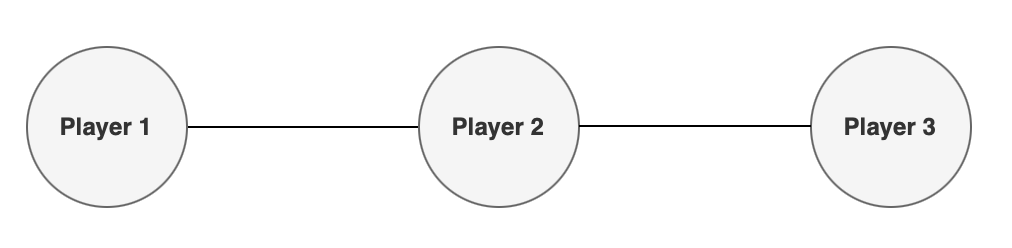
\includegraphics[width = 0.7\textwidth]{Figures/ThreePlayerNetwork.png}
		\caption{\label{fig::ThreePlayerNetwork}}
	\end{figure}

	As an adaptation, we take the example of a three player chain, as depicted in Figure \ref{fig::ThreePlayerNetwork}. In this example, we first assume that the network is simple (i.e. there are no self-loops and $w^{\mu \mu} = 0$). The aggregation matrix can be given as

	\begin{equation}
		W = \begin{bmatrix}
			0 & 1 & 0 \\
			w & 0 & 1 - w \\
			0 & 1 & 0
		\end{bmatrix}, \; w \in (0, 1).
	\end{equation}


	We first consider the zero-sum case to show that it does indeed converge to an equilibrium as expected. Note that the zero-sum condition given for the three player chain is given as

	\begin{equation}
		x \cdot A y + y \cdot B (w x + (1-w)z) + z \cdot C y = 0. \hspace{0.5cm} \forall x, y, z \in \Delta_1 \times \Delta_2 \times \Delta_3
	\end{equation}

	in which we use the notation that $x, y, z$ (resp. $A, B, C$) denote the strategies (resp. payoffs) of agents 1, 2 and 3 respectively. This condition is satisfied if we fix $B$ and choose

	\begin{align}
		A & = - w B^T \\
		C & = - (1 - w) B^T. 
	\end{align}

	As such in the following example, we will set $B = B_\beta$ with the choice $\beta \approx 0.576$ and set $A$ and $C$ according to the above with the choice $w \approx 0.288$. The orbits that these payoff matrices generate can be seen in Figure \ref{fig::convergentShapley}, in which, for each player, they converge to the Nash Equilibrium which, for each player, lies in the centre of the simplex.

	Let us now make the slight modification in the definition of C so that

	\begin{equation}
		C  = - (1 - w) B, 
	\end{equation}

	with no alteration to $A$. The modification itself is small, however it results in the zero-sum assumption being violated. With the same choices of $\beta$ and $w$, this results in the periodic orbit seen in Figure \ref{fig::nonconvergentShapley}. Here, the orbits reach a stable limit cycle which to be centred around the interior NE.

	\begin{figure}[t]
		\centering
		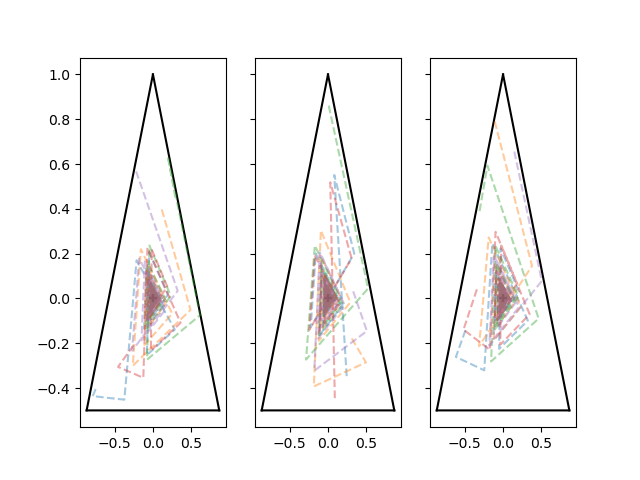
\includegraphics[width = 0.7\textwidth]{Figures/convergentShapley.png}
		\caption{\label{fig::convergentShapley}}
	\end{figure}

	\begin{figure}[t]
		\centering
		\includegraphics[width = 0.7\textwidth]{Figures/nonconvergentShapley.png}
		\caption{\label{fig::nonconvergentShapley}}
	\end{figure}

	As such, we can see that convergent behaviour is not necessarily the norm in the NA-CTFP dynamics. In fact, for the family of games discussed above, we were unable to find non-periodic behaviour for any choice of $\beta$ strictly between 0.5 and 1 for any $w$ between 0.2 and 0.8 (so that the influence of player 1 and player 3 on player 2 is not negligible). This suggests that, far from being rare, in fact NA-CTFP lends itself to an incredibly rich variety of dynamics which can be explored as future work.
	

	\subsection{Addition of Noise}

	The fictitious play process in NA games requires that, at each time step, an agent takes a `measurement' of the aggregate strategy of its neighbours. It is on this measurement that they update their own strategy. It stands to reason that, in real environments, this measurement may be corrupted by noise. As such, we investigate the effect that introducing noise has on CTFP in a zero-sum NA game.

	\ah{To discuss with F before including in the document}.
	

	\section{Discussion}

	\section{Concluding remarks}
\end{document}
